\chapter{Introduction}

Quand vous lancez Super Mario Bros. pour la première fois, le jeu ne vous donne aucune instruction. 
Le premier niveau est savamment conçu pour vous enseigner les règles : sauter sur les ennemis, ramasser les champignons, trouver les secrets cachés, obtenir des pièces, éviter les trous. 
Il n'y a pas de didacticiel. 
Le jeu lui-même est le didacticiel.

Tout le monde peut citer des donjons "classiques" : Tomb of Horrors, La Barrière des Hautes Cimes, Ravenloft, etc.
Mais pour que ces aventures puissent prendre tout leur sens, une sorte d'introduction est nécessaire. 
Tomb of Horrors et Death Frost Doom sont construits comme des réactions à un certain archétype de donjon, qui n'existe pas vraiment, pas sous forme de produit publié, tout du moins.

C'est comme si toutes les aventures à notre disposition étaient des compositions de Bach : les gens écrivent d'incroyables œuvres témoignant d'un génie incomparable, mais il faut que quelqu'un rédige un livre expliquant comment jouer du piano.

Ce donjon est conçu pour être "classique" sans pour autant être truffé de références ou empli de nostalgie. 
Il se conforme à quelques clichés, mais pas tous. Il est également intégralement annoté.

\subsection{Ce module est destiné :}
\begin{enumerate}
  \item Aux MJ expérimentés avec des joueurs débutants ;
  \item Aux MJ souhaitant apprendre à concevoir un donjon ;
  \item Aux MJ expérimentés avec des joueurs vétérans, mais découvrant l'OSR.
\end{enumerate}
Si vous êtes un MJ complètement débutant, vous pouvez toujours utiliser ce donjon et en apprendre beaucoup, mais il
mettra vos compétences à rude épreuve d'entrée de jeu. 
Les joueurs expérimentés pourront probablement l'apprécier eux aussi.

\subsection{Je suis pas d'accord avec...}
Il y a de bonnes chances que les MJ expérimentés soient en désaccord avec certains pièges, leçons ou rencontres de ce
donjon.
Ce n'est pas un souci ! Ce module n'est pas censé être un guide de la "seule bonne façon" de mener un donjon
pour débutants, juste d'une des manières de procéder.

Si vous estimez que la diplomatie est une compétence vitale dès le début, ajoutez un gobelin amical mais froussard nommé
Smée au 7 : Faux Temple (p. 2). 
Si vous pensez que les contraintes temporelles et le sentiment de danger imminent sont importants, faites intervenir des Monstres Errants à tous les niveaux du donjon, pas juste au troisième. 
Si vous n'aimez pas les serpents, remplacez-les par des chèvres. 
Ajoutez des clichés venus du folklore. 
Remplacez les pièges par vos favoris, ou retirez-les complètement.

Au moins, en manifestant votre désaccord, vous apprenez à connaître vos propres préférences. 
C'est toujours utile : savoir ce que l'on n'aime pas est aussi précieux que savoir ce que l'on
aime. 
Qui sait ? Peut-être que ce module vous donnera l'envie d'écrire votre propre "donjon d'apprentissage"

\subsection{Taille du Groupe et Équilibre}
Ce donjon est conçu pour des personnages de niveau 1. 
J'ai tenté le rendre aussi indépendant que possible de tout système de jeu. 
Vous pouvez tout aussi bien mener ce donjon pour un joueur comme pour dix. 
Les rencontres ne sont pas équilibrées. 
Elles n'ont pas de "facteur de puissance". 
Le combat n'est que peu récompensé, mais l'exécution réussie d'un bon plan l'est grandement.

La quantité de trésor est basée sur l'idée que 200 PO sont suffisants pour faire monter un personnage de niveau. 
En arrivant au bout de ce donjon, les PJ survivants devraient avoisiner le niveau 2 voire 3, en supposant un taux standard d'attrition, perte et panique. 
Ajustez la valeur du trésor en conséquence. 
Les grands groupes auront moins de mal (et récupéreront moins de trésor par PJ).
Un joueur solo parvenant à survivre deviendra riche.

La puissance des coups est prévue pour des PJ ayant entre 4 et 16 points de vie, équipés de dagues causant 1d6 dégâts.
Les jets de sauvegarde sont décrits de façon générique (jet de sauvegarde contre le poison, pour esquiver...).

Un groupe de PJ de niveau moyen, joué par des joueurs expérimentés, pourrait venir à bout de ce donjon en un temps
record. 
Il est tout de même possible qu'ils s'amusent. 
Un groupe de PJ de bas niveau joué par des joueurs débutants devrait passer un très bon moment, du moins je l'espère.

En fonction du style de jeu, de la vitesse de progression, des aventures annexes, du temps passé en ville et autres digressions, l'exploration exhaustive de ce donjon peut se compléter en 12 à 24 heures de jeu. 
La durée du Niveau 1 est adaptée à une courte première session précédée d'une création de personnages.

\subsection{Avant de Commencer}
\begin{enumerate}
  \item Lisez le module dans son intégralité.
  \item Prenez note de ce que vous aimez et n'aimez pas.
  \item Imprimez les pages 1 à 17 ainsi que la carte (p. III).
  \item Remplacez les monstres des pages 12 à 14 avec ceux du système choisi.
  \item Ajustez la valeur des trésors autant que nécessaire.
\end{enumerate}

\subsection{Appâter les PJ}
Voici quelques moyens d'amener les PJ au donjon, pour peu qu'ils soient sur la paille et qu'ils sachent que les tombes
contiennent souvent des trésors. 
Vous pouvez placer ce donjon n'importe où.

\begin{enumerate}
  \item Ils trouvent une vieille carte menant à une sépulture tombée dans l'oubli.
  \item Un glissement de terrain révèle l'entrée de la tombe.
  \item Les gobelins (p. 13) kidnappent un proche des PJ.
  \item Les expériences de Xiximantre (p. 13) induisent en eux d'étranges rêves.
  \item Ils tombent sur l'entrée du tombeau alors qu'ils s'occupent d'un problème qui n'a rien à voir.
  \item Un puissant commanditaire les envoie explorer la tombe nouvellement découverte.
\end{enumerate}

\subsection{Leçons}
De petits encadrés didactiques sont parsemés au gré du texte.
Chaque salle, rencontre ou piège est conçu pour enseigner aux nouveaux joueurs (et nouveaux MJ) une leçon pertinente. Certaines d'entre elles sont d'ordre général, tandis que d'autres sont spécifiques à ce donjon. 
La structure, la nature et les dangers du donjon deviennent peu à peu prévisibles et exploitables. 
Les leçons peuvent paraître triviales aux MJ expérimentés, mais je pense que leur présence reste utile malgré
tout.

\subsection{Structure}
La Tombe des Rois Serpents est un donjon enterré divisé en trois niveaux et quatre zones thématiques. 
J'ai inclus des descriptions minimales dans le texte et l'Index des Salles (p. 16). 
Il n'y a pas de paragraphes "à lire à voix haute".

\subsubsection{Niveau 1 : La Fausse Tombe}
Introduit les bases de la conception et exploration de donjon en 7 salles. 

Cette section est pile de la bonne longueur pour une première session, pourvu que la création de personnages ait été rapide et que vous ayez donné aux PJ une bonne raison d'explorer la tombe.

\subsubsection{Niveau 2 : La Tombe Supérieure}
Toujours linéaire, mais avec plus de pièces annexes et quelques dangers environnementaux.
Le chemin "vers l'avant" est toujours clair, mais les salles annexes sont tentantes. 
C'est ici que les leçons du Niveau 1 sont évaluées et mises en pratique.

Cet étage devrait prendre 2 ou 3 sessions à explorer, et peut requérir un trajet de retour à la civilisation pour faire le plein.

\subsubsection{Niveau 3 : La Tombe Inférieure}
Il y a deux chemins principaux "horizontaux" et trois "verticaux". 
Le donjon bifurque et reboucle. 
Il est possible de remonter à la surface comme de plonger plus profond. 
Ou même de revenir de là où l'on est parti. 
Cet étage est indubitablement plus dangereux que les précédents. 

La diplomatie et le troc font également leur apparition, de même que les monstres errants. 
Vous pouvez explorer les niveaux 1 et 2 à votre rythme, mais passer trop de temps au Niveau 3 revient à prendre des risques inconsidérés.

La conclusion de cet étage est ouverte : vous pouvez ajouter du contenu pour étendre ce donjon autant que vous le souhaitez. 
Arrivé là, si vous êtes un nouveau MJ ou débutant en jeux OSR, vous devriez être prêt à écrire votre propre donjon.

\subsection{Zones Thématiques}
\subsubsection{La Fausse Tombe}
Symbolise la joie de la découverte, le moment où l'on se dit "Oh ! Je vois !" et l'anticipation du trésor à venir.
Assurez-vous de féliciter tout joueur parvenant à déduire qu'il s'agit d'une fausse tombe : l'astuce se doit d'être récompensée. 
Le donjon devient de plus en plus étrange au fur et à mesure de la descente. 
Au début, on force des cercueils de bois pour voler de petites amulettes. 
À la fin, on se retrouve à fouiller des déchets de gobelins fongiques pour trouver une couronne, à négocier avec un homme-serpent décédé, ou à convoyer des coffres d'or jusqu'à la surface.

Décrivez cette zone avec des mots comme "branlant", "décrépi" et "humide".
C'est une vieille cave. 
De petites racines blanches pendent du plafond pour venir lécher le sol. 

\subsubsection{La Vraie Tombe}
Représente le pouvoir et les menaces implicites. 
Des statues veillent. 
Des choses tressaillent dans leurs cercueils scellés. 
Des lézards géants vous traquent dans l'obscurité, des sorciers immortels proposent des pactes indicibles et d'invincibles mucus morts-vivants serpentent à votre poursuite.

Décrivez cette zone avec des mots comme "énorme", "menaçant" et "froid". 
C'est l'\oe uvre d'une civilisation bien plus ancienne, sage et cruelle que celle des PJ. 
Plus ils s'enfoncent profondément, plus la tension devrait les rendre nerveux.

\subsubsection{Le Gouffre}
Incarne l'inconnu, et ses promesses.
Il pourrait y avoir n'importe quoi en bas. 
Le centre de la Terre. 
Des hommes-serpents vivant toujours paisiblement dans les profondeurs. 
C'est la toile vierge du module, sur laquelle le MJ peut venir ajouter ce que bon lui semble.

Décrivez le gouffre avec des mots comme "sans fond", "vertigineux, comme si le monde entier s'écroulait" et "résonnant
de lointains mais persistants échos, si vous êtes patients".

Les PJ ne devraient pas vouloir passer plus de temps que nécessaire au bord de l'abîme.

\subsubsection{Les Terriers Gobelins}
Les Gobelins Fongiques sont le miroir des PJ, leur opposé.
Ils se complaisent dans la crasse, revivent sans cesse et commettent toujours les mêmes erreurs. 
Ils sont affamés, stupides, superstitieux et meurtriers, mais néanmoins attachants. 
Les terriers sont l'irruption d'un barbarisme bruyant et enthousiaste dans la civilisation froide et moribonde.

Décrivez les terriers tant par le bruit que par l'odeur. 
Ça pue.
Vous allez puer si vous vous attardez ici, et la Tombe des Rois Serpents n'est pas pourvue de bains. 
Des petits yeux de gobelins dans la pénombre. 
Des dents cliquetantes et des couteaux aiguisés.

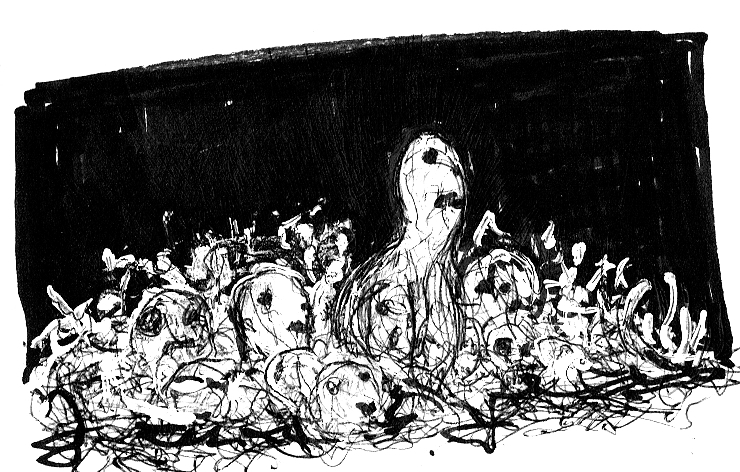
\includegraphics[width=\columnwidth]{pics/goblin_pit.jpg}